%%
%% Automatically generated file from DocOnce source
%% (https://github.com/doconce/doconce/)
%% doconce format latex hw9.do.txt --no_mako
%%
% #ifdef PTEX2TEX_EXPLANATION
%%
%% The file follows the ptex2tex extended LaTeX format, see
%% ptex2tex: https://code.google.com/p/ptex2tex/
%%
%% Run
%%      ptex2tex myfile
%% or
%%      doconce ptex2tex myfile
%%
%% to turn myfile.p.tex into an ordinary LaTeX file myfile.tex.
%% (The ptex2tex program: https://code.google.com/p/ptex2tex)
%% Many preprocess options can be added to ptex2tex or doconce ptex2tex
%%
%%      ptex2tex -DMINTED myfile
%%      doconce ptex2tex myfile envir=minted
%%
%% ptex2tex will typeset code environments according to a global or local
%% .ptex2tex.cfg configure file. doconce ptex2tex will typeset code
%% according to options on the command line (just type doconce ptex2tex to
%% see examples). If doconce ptex2tex has envir=minted, it enables the
%% minted style without needing -DMINTED.
% #endif

% #define PREAMBLE

% #ifdef PREAMBLE
%-------------------- begin preamble ----------------------

\documentclass[%
oneside,                 % oneside: electronic viewing, twoside: printing
final,                   % draft: marks overfull hboxes, figures with paths
10pt]{article}

\listfiles               %  print all files needed to compile this document

\usepackage{relsize,makeidx,color,setspace,amsmath,amsfonts,amssymb}
\usepackage[table]{xcolor}
\usepackage{bm,ltablex,microtype}

\usepackage[pdftex]{graphicx}

\usepackage[T1]{fontenc}
%\usepackage[latin1]{inputenc}
\usepackage{ucs}
\usepackage[utf8x]{inputenc}

\usepackage{lmodern}         % Latin Modern fonts derived from Computer Modern

% Hyperlinks in PDF:
\definecolor{linkcolor}{rgb}{0,0,0.4}
\usepackage{hyperref}
\hypersetup{
    breaklinks=true,
    colorlinks=true,
    linkcolor=linkcolor,
    urlcolor=linkcolor,
    citecolor=black,
    filecolor=black,
    %filecolor=blue,
    pdfmenubar=true,
    pdftoolbar=true,
    bookmarksdepth=3   % Uncomment (and tweak) for PDF bookmarks with more levels than the TOC
    }
%\hyperbaseurl{}   % hyperlinks are relative to this root

\setcounter{tocdepth}{2}  % levels in table of contents

% Tricks for having figures close to where they are defined:
% 1. define less restrictive rules for where to put figures
\setcounter{topnumber}{2}
\setcounter{bottomnumber}{2}
\setcounter{totalnumber}{4}
\renewcommand{\topfraction}{0.95}
\renewcommand{\bottomfraction}{0.95}
\renewcommand{\textfraction}{0}
\renewcommand{\floatpagefraction}{0.75}
% floatpagefraction must always be less than topfraction!
% 2. ensure all figures are flushed before next section
\usepackage[section]{placeins}
% 3. enable begin{figure}[H] (often leads to ugly pagebreaks)
%\usepackage{float}\restylefloat{figure}

% prevent orhpans and widows
\clubpenalty = 10000
\widowpenalty = 10000

% --- end of standard preamble for documents ---


% insert custom LaTeX commands...

\raggedbottom
\makeindex
\usepackage[totoc]{idxlayout}   % for index in the toc
\usepackage[nottoc]{tocbibind}  % for references/bibliography in the toc

%-------------------- end preamble ----------------------

\begin{document}

% matching end for #ifdef PREAMBLE
% #endif

\newcommand{\exercisesection}[1]{\subsection*{#1}}


% ------------------- main content ----------------------



% ----------------- title -------------------------

\thispagestyle{empty}

\begin{center}
{\LARGE\bf
\begin{spacing}{1.25}
PHY321: Classical Mechanics 1
\end{spacing}
}
\end{center}

% ----------------- author(s) -------------------------

\begin{center}
{\bf Homework 9, due Friday  April 28 (note changed deadline)${}^{}$} \\ [0mm]
\end{center}

\begin{center}
% List of all institutions:
\end{center}
    
% ----------------- end author(s) -------------------------

% --- begin date ---
\begin{center}
Apr 20, 2022
\end{center}
% --- end date ---

\vspace{1cm}


\paragraph{Practicalities about  homeworks and projects.}
\begin{enumerate}
\item You can work in groups (optimal groups are often 2-3 people) or by yourself. If you work as a group you can hand in one answer only if you wish. \textbf{Remember to write your name(s)}!

\item Homeworks are available  the week before the deadline. 

\item How do I(we)  hand in?  Due to the corona virus and many of you not being on campus, we recommend that you scan your handwritten notes and upload them to D2L. If you are ok with typing mathematical formulae using say Latex, you can hand in everything as a single jupyter notebook at D2L. The numerical exercise(s) should always be handed in as a jupyter notebook by the deadline at D2L. 
\end{enumerate}

\noindent
\paragraph{Introduction to homework 9.}
This week's exercises focus on solving
two-body  problems with central forces and the Lagrangian formalism (exercise 5). There are no numerical exercises. 
The first four exercises are examples taken from our discussions of two-body problems and the relevant theory is to be found in chapter 8 of Taylor. The last exercise involves chapters 6 and 7 of Taylor.

\paragraph{Exercise 1: Attractive Potential (10pt).}
Consider a particle in an attractive potential
\[
V(r)=-\alpha/r.
\]

The quantity $r$ is the absolute value of the relative position. We
will use the reduced mass $\mu$ and the angular momentum $L$, as
discussed during the lectures. With the transformation of a two-body
problem to the center-of-mass frame, the actual equations look like an
\emph{effective} one-body problem. The energy of the system is $E$ and the
minimum of the effective potential is $r_{\rm min}$.

The analytical solution to the radial equation of motion is
\[
r(\phi) = \frac{1}{\frac{\mu\alpha}{L^2}+A\cos{(\phi)}}.
\]

Find the value of $A$. Hint: Use the fact that at $r_{\rm min}$
there is no radial kinetic energy and $E=-\alpha/r_{\rm min}+L^2/2mr_{\rm min}^2$.

\paragraph{Exercise 2 (20pt) Inverse-square force.}
Consider again the same effective potential as in exercise 1. This leads to an attractive inverse-square-law force, $F=-\alpha/r^2$. Consider a particle of mass $m$ with angular momentum $L$. Taylor sections 8.4-8.7 are relevant background material.  See also the harmonic oscillator potential from hw8. The equation of motion for the radial degrees of freedom is (see also hw8) in the center-of-mass frame in two dimensions with $x=r\cos{(\phi)}$ and $y=r\sin{(\phi)}$ and
$r\in [0,\infty)$, $\phi\in [0,2\pi]$ and $r=\sqrt{x^2+y^2}$ are given by
\[
\ddot{r}=-\frac{1}{m}\frac{dV(r)}{dr}+r\dot{\phi}^2,
\]
and
\[
\dot{\phi}=\frac{L}{m r^2}.
\]
Here $V(r)$ is any central force which depends only on the relative coordinate.

\begin{itemize}
\item 2a (5pt)  Find the radius of a circular orbit by solving for the position of the minimum of the effective potential. 

\item 2b (5pt) At the minimum, the radial velocity is zero and it is only the \href{{https://en.wikipedia.org/wiki/Centripetal_force}}{centripetal velocity} which is nonzero. This implies that $\ddot{r}=0$.  What is the angular frequency, $\dot{\theta}$, of the orbit? Solve this by setting $\ddot{r}=0=F/m+\dot{\theta}^2r$.

\item 2c (5pt) Find the effective spring constant for the particle at the minimum.

\item 2d (5pt) What is the angular frequency for small vibrations about the minimum? How does this compare with the answer to 2b?
\end{itemize}

\noindent
\paragraph{Exercise 3, Inverse-square force again (10pt).}
Consider again a  particle of mass $m$ in the same attractive potential, $V(r)=-\alpha/r$, with angular momentum $L$ with just the right energy so that

\[
A=m\alpha/L^2
\]
where $A$ comes from the expression
\[
r=\frac{1}{(m\alpha/L^2)+A\cos{(\phi)}}.
\]
The trajectory can then be rewritten as
\[
r=\frac{2r_0}{1+\cos\theta},~~~r_0=\frac{L^2}{2m\alpha}.
\]

\begin{itemize}
\item 3a (5pt) Show that for this case the total energy $E$ approaches zero.

\item 3b (5pt) With zero energy $E=0$, write this trajectory in a more recognizable parabolic form, that is express $x_0$ and $R$ in terms of $r_0$ using 
\end{itemize}

\noindent
\[
x=x_0-\frac{y^2}{R}.
\]

\paragraph{Exercise 4, parabolic and hyperbolic orbits (10pt).}
The solution to the radial function for an inverse-square-law force, see for example Taylor equation (8.59) or the equation above, is
\[
r(\phi) = \frac{c}{1+\epsilon\cos{(\phi)}}.
\]

For $\epsilon=1$ (or the energy $E=0$) the orbit reduces to a parabola as we saw in the previous exercise,
while for $\epsilon > 1$ (or energy positive) the orbit becomes a hyperbola. The equation for a hyperbola in Cartesian coordinates is
\[
\frac{(x-\delta)^2}{\alpha^2}-\frac{y^2}{\beta^2}=1.
\]
For a hyperbola, identify the constants $\alpha$, $\beta$ and $\delta$ in terms of the constants $c$ and $\epsilon$ for $r(\phi)$. 

\paragraph{Exercise 5 (40pt), Pendulum and Lagrangians (Taylor chapters 6-7).}
A mathematical pendulum consists of a point mass $m$ suspended by a massless thread/rod of length $l$ in a gravitational field, as shown in the figure here. The constraining force is labeled by $\bm{T}$
and the gravitational force is labeled $\bm{F}_g$.

\vspace{6mm}

% inline figure
\centerline{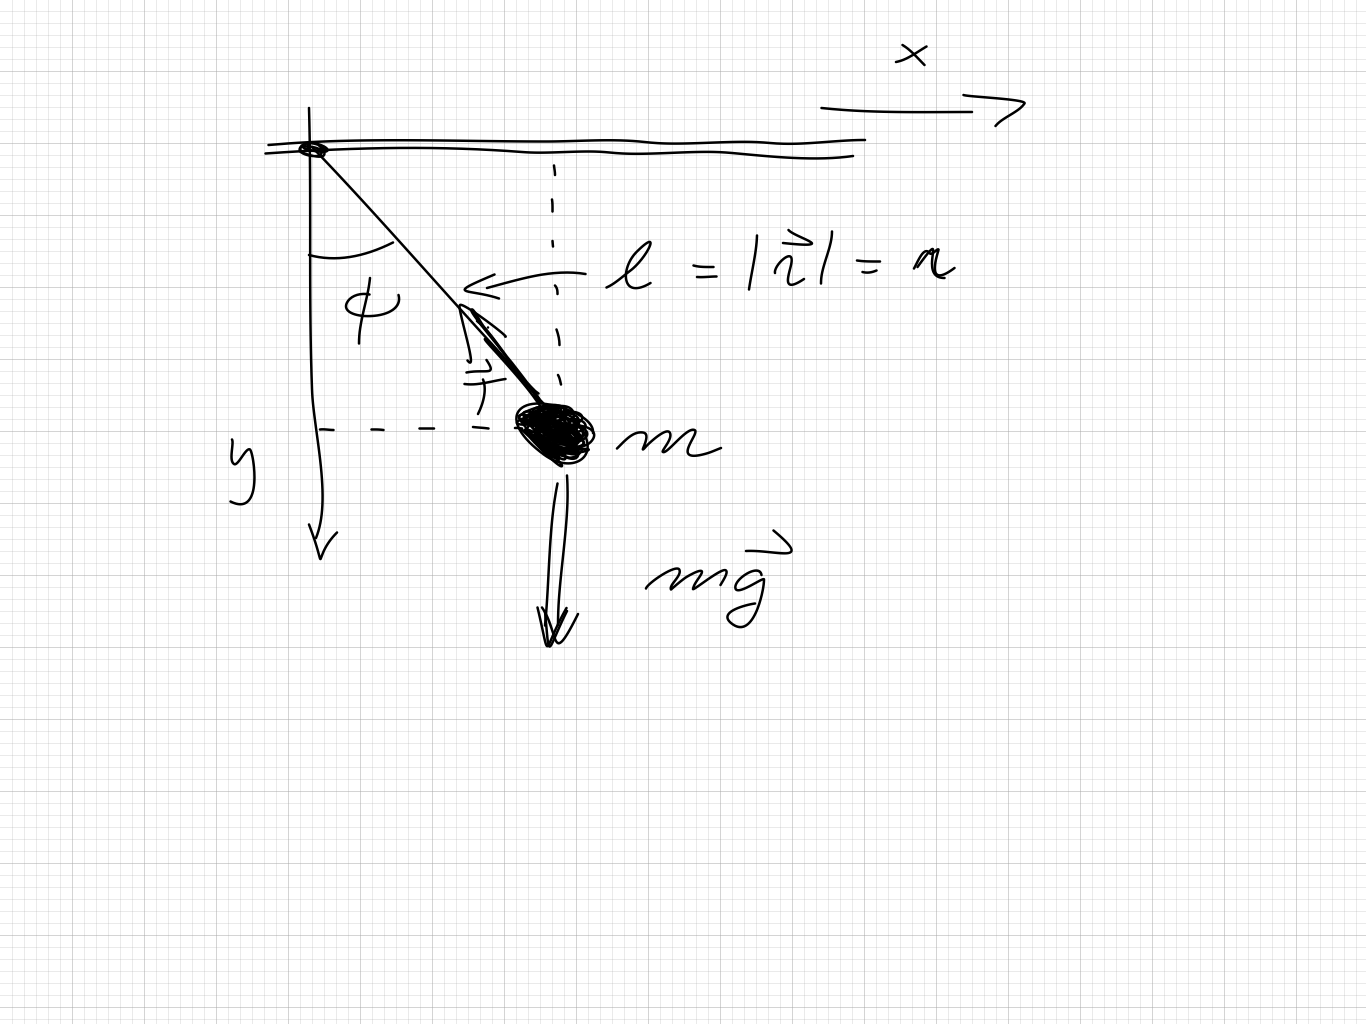
\includegraphics[width=0.6\linewidth]{figures/Simplependulum.png}}

\vspace{6mm}

We assume that the length $l$ is constant and we define the coordinates involved as

\[
\bm{r} = l\sin(\phi)\bm{\hat{x}}+l\cos(\phi)\bm{\hat{y}},
\]
where $\bm{\hat{x}}$ and $\bm{\hat{y}}$ are the unit vectors in the $x$ and $y$ directions, respectively.

\begin{itemize}
\item \textbf{5a (10pt):} Set up the forces acting on the system and show that the equation of motion is $m\ddot{\bm{r}}=\bm{F}_g+\bm{T}$.

\item \textbf{5b (10pt):} Show that you can rewrite the above equation of motion as two independent equations of motion, one for $\phi$ and one for the constraining force. Show that these equations are $\ddot{\phi}(t)=-\omega_0^2\sin{(\phi(t))}$ with $\omega_0^2=g/l$ and $T=ml\dot{\phi}^2+mg\cos{(\phi)}$.
\end{itemize}

\noindent
The equation for $\phi$ is a second-order differential equation
\[
\ddot{\phi}(t)=-\omega_0^2\sin{(\phi(t))}.
\]

This equation can be solved analytically if we assume that the angle $\phi$ is very small. Then we can approximate our equation as

\[
\ddot{\phi}(t)=-\omega_0^2\phi(t).
\]

\begin{itemize}
\item \textbf{5c (5pt):} Find the analytical solution for the last equation. Hint, look back at the solutions for the simple harmonic oscillator problem in one dimension in for example homework 8.

\item \textbf{5d (5pt):} Find the expressions for the kinetic and potential energies in terms of the variables $r$ and $\phi$. 

\item \textbf{5e (10pt):} With the potential $V$  and kinetic $T$ energies, define the Lagrangian for the mathematical pendulum discussed here. Add the constraint $r=l$ via a Lagrange multiplier $\lambda$ and derive the equations of motion. Show that these result in  $\ddot{\phi}(t)=-\omega_0^2\sin{(\phi(t))}$ with $\omega_0^2=g/l$ and $\lambda=ml\dot{\phi}^2+mg\cos{(\phi)}$.  How would you interpret $\lambda$? 
\end{itemize}

\noindent
\paragraph{Classical Mechanics Extra Credit Assignment: Scientific Writing and attending Talks.}
The following gives you an opportunity to earn \textbf{five extra credit
points} on each of the remaining homeworks and \textbf{ten extra credit points}
on the midterms and finals.  This assignment also covers an aspect of
the scientific process that is not taught in most undergraduate
programs: scientific writing.  Writing scientific reports is how
scientist communicate their results to the rest of the field.  Knowing
how to assemble a well written scientific report will greatly benefit
you in you upper level classes, in graduate school, and in the work
place.

The full information on extra credits is found at \href{{https://github.com/mhjensen/Physics321/blob/master/doc/Homeworks/ExtraCredits/}}{\nolinkurl{https://github.com/mhjensen/Physics321/blob/master/doc/Homeworks/ExtraCredits/}}. There you will also find examples on how to write a scientific article. 
Below you can also find a description on how to gain extra credits by attending scientific talks.

This assignment allows you to gain extra credit points by practicing
your scientific writing.  For each of the remaining homeworks you can
submit the specified section of a scientific report (written about the
numerical aspect of the homework) for five extra credit points on the
assignment.  For the two midterms and the final, submitting a full
scientific report covering the numerical analysis problem will be
worth ten extra points.  For credit the grader must be able to tell
that you put effort into the assignment (i.e.~well written, well
formatted, etc.).  If you are unfamiliar with writing scientific
reports, \href{{https://github.com/mhjensen/Physics321/blob/master/doc/Homeworks/ExtraCredits/IntroductionScientificWriting.md}}{see the information here}

The following table explains what aspect of a scientific report is due
with which homework.  You can submit the assignment in any format you
like, in the same document as your homework, or in a different one.
Remember to cite any external references you use and include a
reference list.  There are no length requirements, but make sure what
you turn in is complete and through.  If you have any questions,
please contact Julie Butler at butler@frib.msu.edu.


\begin{quote}
\begin{tabular}{ccc}
\hline
\multicolumn{1}{c}{ HW/Project } & \multicolumn{1}{c}{ Due Date } & \multicolumn{1}{c}{ Extra Credit Assignment } \\
\hline
HW 3               & 2-8           & Abstract                   \\
HW 4               & 2-15          & Introduction               \\
HW 5               & 2-22          & Methods                    \\
HW 6               & 3-1           & Results and Discussion     \\
\textbf{Midterm 1} & \textbf{3-12} & \emph{Full Written Report} \\
HW 7               & 3-22          & Abstract                   \\
HW 8               & 3-29          & Introduction               \\
HW 9               & 4-5           & Results and Discussion     \\
\textbf{Midterm 2} & \textbf{4-16} & \emph{Full Written Report} \\
HW 10              & 4-26          & Abstract                   \\
\textbf{Final}     & \textbf{4-30} & \emph{Full Written Report} \\
\hline
\end{tabular}
\end{quote}

\noindent
You can also gain extra credits if you attend scientific talks.
This is described here.

\paragraph{Integrating Classwork With Research.}
This opportunity will allow you to earn up to 5 extra credit points on a Homework per week. These points can push you above 100\% or help make up for missed exercises.
In order to earn all points you must:

\begin{enumerate}
\item Attend an MSU research talk (recommended research oriented Clubs is  provided below)

\item Summarize the talk using at least 150 words

\item Turn in the summary along with your Homework.
\end{enumerate}

\noindent
Approved talks:
Talks given by researchers through the following clubs:
\begin{itemize}
\item Research and Idea Sharing Enterprise (RAISE)​: Meets Wednesday Nights Society for Physics Students (SPS)​: Meets Monday Nights

\item Astronomy Club​: Meets Monday Nights

\item Facility For Rare Isotope Beam (FRIB) Seminars: ​Occur multiple times a week
\end{itemize}

\noindent

% ------------------- end of main content ---------------

% #ifdef PREAMBLE
\end{document}
% #endif

